%\documentclass[a4paper, english,10pt]{article}
%\documentclass[english,10pt, oneside, draft, a4paper]{report}
\documentclass[english,10pt, oneside, a4paper]{scrreprt}
%\usepackage[b5paper, layout=b5paper, textwidth=12cm, twoside,bindingoffset=1cm,outer=2cm,inner=2cm,includefoot,bmargin=3cm]{geometry}
\usepackage[a4paper, layout=a4paper, textwidth=12cm, bindingoffset=1cm,outer=2cm,inner=2cm,includefoot,bmargin=3cm]{geometry}
\usepackage[english]{babel}
\usepackage[utf8]{inputenc}
\usepackage[T1]{fontenc}
\usepackage{float}
\usepackage{subfig}
\usepackage{multirow}
\usepackage{tabularx}
\usepackage{perpage} % For å få fotnotenummerering til å starte på nytt for hver side
\usepackage{graphicx}
\graphicspath{{grafikk/}}
\usepackage[export]{adjustbox} %In including a figure, add "center" as a flag

\usepackage{epstopdf}
\usepackage{varioref}
\usepackage{listings} % For å vise frem kode på en bra måte
\usepackage{textgreek}
%\usepackage{tikz,pgfplots} % For å plotte Matlab figurer på en god måte
\usepackage{amsmath} % For å tilpasse ligninger til å vises over flere linjer
\usepackage{pdfpages} % For å legge til pdf i appendix delen
\usepackage{rotating}
\usepackage{hyperref} % [pdfborder=0]{hyperref} to remove borders around
% pdf-links.
%\usepackage[text={6.2in,9.5in},centering]{geometry}
\usepackage{mathtools}
\usepackage{color} % Farger i dokumentet

\usepackage{dialogue}
\usepackage[section]{placeins}

\linespread{1.5}

% \lstset{frame=shadowbox, rulesepcolor=\color{black}}
\lstset{numbers=left, frame=single, tabsize=2, breaklines=true}

\DeclarePairedDelimiter\abs{\lvert}{\rvert}%
\DeclarePairedDelimiter\norm{\lVert}{\rVert}%

\makeatletter
\let\oldabs\abs
\def\abs{\@ifstar{\oldabs}{\oldabs*}}
%
\let\oldnorm\norm
\def\norm{\@ifstar{\oldnorm}{\oldnorm*}}
\makeatother


\DeclareMathSymbol{\comma}{\mathpunct}{letters}{"3B} % Legger inn kommandoen \comma som komma i math mode

\hypersetup{%
    pdfborder = {0 0 0}
}

%\usepackage{endnotes}
%\usepackage[portrait, pdftex]{geometry}

\newcommand{\HRule}{\rule{\linewidth}{0.5mm}}
\pretolerance = 1414
\tolerance = 1414

\MakePerPage{footnote} % For å få fotnotenummerering til å starte på nytt for hver side
\labelformat{equation}{equation~(#1)}
\labelformat{figure}{figure~{#1}}
\labelformat{table}{table~{#1}}


% ########################################## 
%			Beginning of document
% ########################################## 

\begin{document}

% \title{Designing a software architecture for a motorsport driver information system}
% \author{Magnus Bae and Magnus Krane\\ NTNU}
% \date{December 2013}
% \maketitle
%% \title{Designing a software architecture for a motorsport driver information system}
% \author{Magnus Bae and Magnus Krane\\ NTNU}
% \date{December 2013}
% \maketitle

\title{Piloting map service for navigating in punctuality analysis for trains}
 
\date{ June 17, 2014}


\begin{titlepage}
\begin{center}

\vspace{10mm}
\includegraphics[width=0.55\textwidth]{logo_ntnu_eng.png}~\\[1cm]
 \vspace{40mm}

\makeatletter
    \parindent \z@
    \reset@font
    \vskip 40\p@
    \par
    \hrule height 2pt
    \par
    \vskip 4\p@
    \huge \@title
    \vskip 6\p@
    \par
    \hrule height 2pt
    \par
    \begin{flushright}
      \large \@date \par
    \end{flushright}
    \vskip 100\p@
 \vspace{20mm}
\begin{minipage}{0.4\textwidth}
\begin{flushleft} \large
\centerline{Magnus Krane}
~\\
\centerline{Supervisor:}
\centerline{Sobah Petersen}
\centerline{Co-supervisor:}
\centerline{Andreas Amdahl Seim - SINTEF}
\end{flushleft}
\end{minipage}
% \begin{minipage}{0.4\textwidth}
% \begin{flushright} \large
% \emph{Landsby:}\\
% Byggelandsbyen, \textsc{TTK4850}\\
% \emph{Fagl\ae rer:} \\
% F\o rsteamanuensis Sverre \textsc{Hendseth}\\
% \end{flushright}
% \end{minipage}
 
\vfill
\end{center}
\end{titlepage}


\setcounter{tocdepth}{5}
\setcounter{secnumdepth}{5}

%\includepdf[pages={-}]{signert_masterbeskrivelse.pdf} Eksempel på hvordan du legger inn pdf

\setcounter{page}{0}
\pagenumbering{roman}
% \pagedial{empty}

%Does the report contain the necessary elements as 
%abstract/summary, 
%table of 
%contents, 
%introduction, etc. in an appropriate form 

%starting point/objectives, 
%what is done and the 
%conclusions/results, and to maintain this overview throughout the reading. 

% #### Other stuff from the template

% \title{Designing a software architecture for a motorsport driver information system}
% \author{Magnus Bae and Magnus Krane\\ NTNU}
% \date{December 2013}
% \maketitle

\title{Piloting map service for navigating in punctuality analysis for trains}
 
\date{ June 17, 2014}


\begin{titlepage}
\begin{center}

\vspace{10mm}
\includegraphics[width=0.55\textwidth]{logo_ntnu_eng.png}~\\[1cm]
 \vspace{40mm}

\makeatletter
    \parindent \z@
    \reset@font
    \vskip 40\p@
    \par
    \hrule height 2pt
    \par
    \vskip 4\p@
    \huge \@title
    \vskip 6\p@
    \par
    \hrule height 2pt
    \par
    \begin{flushright}
      \large \@date \par
    \end{flushright}
    \vskip 100\p@
 \vspace{20mm}
\begin{minipage}{0.4\textwidth}
\begin{flushleft} \large
\centerline{Magnus Krane}
~\\
\centerline{Supervisor:}
\centerline{Sobah Petersen}
\centerline{Co-supervisor:}
\centerline{Andreas Amdahl Seim - SINTEF}
\end{flushleft}
\end{minipage}
% \begin{minipage}{0.4\textwidth}
% \begin{flushright} \large
% \emph{Landsby:}\\
% Byggelandsbyen, \textsc{TTK4850}\\
% \emph{Fagl\ae rer:} \\
% F\o rsteamanuensis Sverre \textsc{Hendseth}\\
% \end{flushright}
% \end{minipage}
 
\vfill
\end{center}
\end{titlepage}


%\addcontentsline{toc}{section}{Preface}
\section*{Preface}

		XXX


\mbox{}\\[10pc]
\begin{center}
Trondheim, July 02, 2014\\[1pc]
\vspace{15 mm}
Magnus Krane
\end{center}

\clearpage

%\addcontentsline{toc}{section}{Abstract}
\section*{Abstract}

In a complex system such as the Norwegian railway network, there are much that
can affect a trains punctuality. The undertakers strive to achieve higher and
higher punctuality. The infrastructure owner, Jernbaneverket, strive for
minimal downtime on the railway network.

\clearpage

%\addcontentsline{toc}{section}{Norwegian Summary}
\section*{Norwegian summary}

		XXX
\clearpage


\renewcommand\listfigurename{List of Figures}
\listoffigures
\clearpage
\renewcommand\listtablename{List of Tables}
\listoftables
\clearpage
\renewcommand\contentsname{Table of Contents}
\tableofcontents

\setcounter{page}{0}
\pagenumbering{arabic}


% !TEX root=../thesis.tex

\chapter{Introduction}
% chapter Introduction
\label{chapter:introduction}

%This thesis discusses the analysis of train delays and the visualization of these delays. The project involves developing a prototype map visualization of delays based on train routes in Norway. Such features as the ability to scroll through a certain time period (which will be selectable), both backwards and forwards will be implemented. The prototype enables studying of information aggregated through a hierarchy of stakeholders, and study the stakeholders need for different types of information.

In this chapter we introduce the problem which we discuss in this thesis.
%TODO
We will first present the research question which we will answer with the help
of the method presented in \Ref{cha:research_questions_and_method} \nameref{cha:research_questions_and_method}.

\section{Background and motivation} % (fold)
\label{sec:background_and_motivation}
In a railway network there are trains driven most of the time in order to meet
public demand for both passenger and cargo transport. The companies
responsible for the transportation strives for more efficient capacity usage
and increased punctuality. The Norwegian National Rail Administration 
(Jernbaneverket \cite{jernbaneverketAbout}) collects data about every train
driven in the railway network and external events affecting the railway, such 
as flooding. By study of the collected data, users throughout the companies can
plan improvements to be performed on the infrastructure and the usage of the
railway.\\

Most of the data collected is kept in different sets throughout the different
companies with a non-coherent definition of data-fields. The structuring of 
the data sets makes comparison for different users difficult. Different users
throughout the companies have different needs when studying the data, some have
the need for a large geographical area and a low level of data resulting in a
overview, while others need the opposite. \\

The work performed in this thesis is performed in collaboration with the SINTEF
project "PRESIS" \cite{sintefPresis}. The PRESIS\cite{sintefPresis} project is 
a collaboration between SINTEF\cite{sintef}, Transportøkonomisk Institutt
\cite{transportOkonomiskInstitutt}, NTNU\cite{ntnu}, Jernbaneverket(
\Ref{sub:subsection_jernbaneverket}) and the train operators Cargonet (
\Ref{sub:subsection_cargonet}), NSB\cite{nsbForside}, and Flytoget
\cite{flytoget}. The aim of the project is to systematically improve the 
precision level in the railway system by developing methods, tools, and 
processes.

% section background_and_motivation (end)

\section{Research Question and Goals} % (fold)
\label{sec:intro_research_question}
In this section we will introduce the research question and goals which we 
answer in this thesis.\\

A system which allows the user to select between different type of information
to be presented, and at the same time the is aware of the stakeholders that are
relevant to the system, can seem complex. By answering the research question
below, we aimed to produce characteristics which helps define a
stakeholder aware system.\\

\begin{itemize}
	\item \textbf{What are important characteristics for a stakeholder aware 
	method to aggregate over a rich set of data?}
\end{itemize}

As part of answering the research question, we developed a prototype. Using the
research method we produced the following goals for the prototype.

\begin{itemize}
	\item Develop a map based prototype for train analysis.
	\item Sub goals:
	\begin{itemize}
		\item Display dashboard with relevant information accordingly to 
		current zoom level.
		\item Aggregate through statistical data according to current level.
		\item Limit the data visualization within selectable time scales.
		\item Select different type of statistical data to display.
		\begin{itemize}
			\item Display information for traffic density.
			\item Display information for Speed restrictions.
			\item Display information for train crossings.
		\end{itemize}
	\end{itemize}
\end{itemize}

As part of discussing a method for "awareness in presentation", a presentation
of the key parts in the research question is needed. 

By presenting a stakeholder aware method, there are some concerns which needs
to be introduced first. In our problem, we define a stakeholder as a person
within a organizational structure. 

- introdusere problem
- forklare stakeholder problematikk
- rich data set = flere data typer
- prosessere ifølge stakeholder
% section research_question (end)


\section{Stakeholders} % (fold)  
\label{sec:intro_stakeholders}  
As with any project, we had several stakeholders to take into consideration
during the work of this project. A stakeholder is anyone who has a stake in 
the success of the system, which typically have different specific concerns 
that they wish the system to guarantee or optimize 
\cite{Bass:2012:SAP:2392670}.\\

%By presenting a stakeholder aware system, we need to define stakeholders withing the operating domain of the system. 
Stakeholders need to be defined further then just for instance the developers
or project managers, in order to have awareness in how the data is processed 
and presented to the different stakeholders. 
By defining the domain and environment the system will
operate within, further defining of the stakeholders the system will process 
is needed within the domain. When the stakeholders have been defined within 
the domain, their needs and requirements can be defined in a way that the data 
processing methods can take into consideration. \\

When defined within the domain, the stakeholders needs to be organized on a 
structure which enables awareness from the system. During the work of this 
thesis, we present a structure where the stakeholders have been placed in a 
hierarchy according to their areas of responsibility. By organizing a 
hierarchy of the stakeholder, we are able to process the data and limit the 
presentation according to the active stakeholder. 
% section stakeholders (end)

\section{Data Sets} % (fold)
\label{sec:intro_data_sets}
Depending on the system and the stakeholders requirements, the amount of data
to process can quickly grow quite large. As the data required by the
stakeholders involves different types of data, the sets often originates from
different sources. In order to allow the system to process the data according
to the stakeholders, the sets need to be defined in a common structure.
Different companies can for instance have different definitions of the same
data field.
% section data_sets (end)


\section{Aggregation} % (fold)
\label{sec:intro_aggregation}
When the stakeholders have been organized in a data processing friendly
structure as presented in \Vref{sec:intro_stakeholders}, we then aggregate the 
data accordingly. To aggregate data means to replace groups of observations
with summary statistics based on these observations \cite{ wiki:Aggregation}.
By aggregating the data according to the stakeholders, we summarize the data
according to the areas of responsibility. The summarization method used on the 
data are specified by the requirements of the stakeholders. We also present
aggregation through time. Each stakeholder are able to limit the data 
according the level of detail needed, by enabling time aggregation.
\\


% section aggregation (end)

% chapter Introduction (end)

\chapter{Definitions \& abbreviations}
%Abbreviations and definitions
\label{sec:abbriv}
\vspace{5mm}

\begin{description}
\item [GIS] Geographic information system
\item [Regularity]	Jernbaneverket defines regularity as the number of trains that gets run as planed in the time schedule. 
\item [Uptime]	Jernbaneverket states that uptime in regards to punctuality defines from hours of delay caused by infrastructure relative to sum of planed train hours per year. \begin{equation} Uptime =
\frac{\text{Train hours - hours of delay}}{[\text{Train hours}}\times 100 \end{equation}
\end{description}



% !TEX root=../thesis.tex

\begin{flushright}{\slshape 
	I would like to make a case for the car, despite all the manufacturers' 
	claims down the decades,\\
	being the piece of technology that has made the slowest advances 
	towards the clean, safe, digital,\\
	pastel-colored, technology-dominated, communications-driven future that 
	awaits us.\\
	It is still an analogue great lump of metal, a simple machine that we 
	must operate. \\
	Thank God.} \\ \medskip
		--- Richard Hammond \cite{Hammond} 
\end{flushright}


\bigskip

\begingroup
\let\clearpage\relax
\let\cleardoublepage\relax
\let\cleardoublepage\relax


\chapter{Background and State of The Art}

In this chapter we will discuss the background for the project and present 
related theory and research.
We will also spend some time on modern car electronics and sensor systems, and the state of the art for
In Vehicle Information Systems (IVIS) and display technology.
\\
\section{Revolve NTNU}
Revolve NTNU is a student organization which participates in the Formula 
Student competition. Founded in 2010 based on the wish to get more practical 
experience during their studies at NTNU. \cite{Revolve:history} Revolve has competed in Formula Student 
UK (FSUK) and Formula Student Germany (FSG) in both 2012 and 2013. The team is now 
well underway in designing the car for the 2014 competitions. See appendix
\vref{appendix:formula}
for more details about the Formula Student series of competitions.


\subsection{Entries}
The 2012 and 2013 contributions from Revolve both came in the form of a petrol powered race car driven by an internal combustion engine (ICE)
 \cite{Revolve:car13}.
The cars are built to comply with restrictions and demands posed by rules and 
regulations. These regulations set, among others, limits for size of the car, 
requirements for the driver position and power output.
The 2014 contribution, which at time of writing is in the design phase, is going to be a battery powered race car driven by an electric motor \cite{Revolve:car14}.

The choice of an electrically powered drive-train changes some aspects of the 
car compared to using an ICE. Most notably there's not going to be multiple 
selectable gear-ratios, 
but instead one fixed gear ratio. As for sensors and electronics there is not 
a very big change. There are however some changes in instrumentation;
there is no need to
let the driver know he should change gears for instance.  
On the other hand, there will be high density batteries which develops heat and need to be cooled, and there is also a need to inform the driver
of the battery charge level.

\section{Instrumentation and Control}


\subsection{Sensors and control networks}
Both racing  and  personal vehicles are fitted with complex mechanical and electrical
systems being controlled mostly by small embedded computers. For these systems
to be able to perform regulation they need input data about the state of
the surrounding and controlled systems. This data is gathered by means of
sensors registering real-world factors like position, temperature, pressure,
and flow that in turn is feed into the control system.

Sensor systems can also be used to gather data to create meaningful feedback 
for the driver or operator. This is usually visualized through the instruments
located in the dashboard, but can also be conveyed through other means (parking
sensors usually utilize sound).

\begin{figure}[!htbp]
	\includegraphics[width=\textwidth]{human-loopback-control.png}
	\caption{A sensor system where data is used to create feedback for the driver.}
	\label{fig:human-loopback}
\end{figure}

\begin{figure}[!htbp]
	\includegraphics[width=\textwidth]{simple-loopback-control.png}
	\caption{A simple loopback control system.}
	\label{fig:simple-loopback}
\end{figure}
\noindent Traditionally sensors used to be directly wired to the control unit (see \vref{fig:simple-loopback}), but as
system complexity and the
number of sensors grew this made the overall complexity very high. In addition
some sensors are very far away from their control units, examples are sensors 
that detect collisions and wheel speed. The solution to avoid having several 
kilometers of wires is to utilize digital communication buses which allows
components to communicate with each other and significantly reduces the amounts of 
wires needed. It also allows one sensor to input signals to multiple
control systems.
\begin{figure}[!htbp]
	\includegraphics[width=\textwidth]{intermediate-loopback-control.png}
	\caption{A message passing loopback control system. The control unit receives
	message through a sensor network.}
	\label{fig:intermediate-loopback}
\end{figure}

The most significant bus-standard is the Controller Area Network bus
(``CAN-bus'')
that was developed specifically to be used for automotive purposes and is
very error-resilient \cite[1]{can-appnote}.

In a CAN system connected nodes communicate by sending messages (``frames'').
Frames have an id which is also the priority of the message (lower number =
higher priority), if two nodes attempt to send at the same time the frame
with the highest priority will be transported over the bus, the losing node
will retry when the bus is clear. \cite{can-appnote}

The CAN standard is present in the majority of modern cars, which are (more or less) required to
have a CAN-bus through the OBD-II standard \cite{wiki:OBDII}. CAN is also seeing
great adoption in other areas as well. At NTNU CAN is the most emphasized
communication standard in the ``Industrial and Embedded Computer Systems
Design'' course, and is also, coincidentally, the communication standard 
Revolve has decided to
use in their designs. CAN-buses allows easy connection of components and is
also quite fault tolerant, which makes it very applicable for automobile
purposes \cite{can-appnote}.

ISO11898 and ISO11519 describe high- and low-speed interfaces for CAN. 
Together with the CAN-standard these provide the lower 
two layers of the OSI-model \cite{microsoft:osi}. The other layers are 
implementation specific; meaning that routines, package structure, 
and error handling routines are defined by the developers. This means that 
implementations are application specific, but also gives the 
developer room for utilizing the bus the way they see fit. \cite{can-appnote}

\subsection{Digital communication with analog sensors}
Output from a sensor doesn't necessarily make much sense if you view the raw data, 
for instance - a temperature sensor might give outputs between 0 and 5 volts.
Sensors are in their very nature analog\footnote{However digital sensors are
becoming more and more common, they do however still contain the same
components, the difference is that they are packaged together - reducing development
time and physical size of sensor assembly.} and thus requires their output
values to be represented digitally. Although some modern sensors come with
digital outputs, most sensors requires peripheral components that adapt an
output voltage to a level suitable for digitalizing before an analog-to-digital
converter reads the voltage and can communicate it to other digital components,
most commonly a micro controller unit (MCU). The MCU would then take the value
from the sensor, wrap it in a CAN-frame and transmit it on the
CAN-bus, either at its own accord or when requested from another node. \cite[loc. 5020-5203,
5732-7565]{catsoulis:embedded}\cite{can-appnote}
\begin{figure}[!htbp]
	\includegraphics[width=\textwidth]{simple-sensor-and-ad.png}
	\caption{Example of a modern sensor assembly. The sensors analog output is converted to a
	4-bit
	digital signal using an analog/digital converter, its output is read by a
	microcontroller and transmitted over a CAN-network with the use of a
	CAN-tranceiver. Blue lines indicates signal path.}
	\label{fig:simple-sensor}
\end{figure}


\subsection{Electrical noise and protection}
Wires are basically antennas and are susceptible to catching induced currents
from magnetic fields, and also emits their own magnetic fields when current is
applied. Petrol engines use high-voltage components that may create a lot of
noise if not shielded properly. This often results in noisy electrical
environments, something even modern cars struggle with. Automobile electronics
have to be designed to tolerate very high transient voltages. \cite[loc. 2562]{catsoulis:embedded}\footnote{loc. refers to Kindle location. This cannot be compared to ordinary page numbering.}

\subsection{Display Technology}
The standard information system for cars is obviously the dashboard, but it too
has undergone changes and in modern iterations are becoming increasingly
sophisticated. Mercedes have for some years been offering cars with night
vision cameras and a screen overlay in the dashboard \cite{Daimler}. BMW are
offering head-up displays on some of their models, claiming it allows drivers
to process information up to 50\% faster \cite{BMW}.

2012 saw the announcement of Google's ``Glass'' project \cite{nytimes:glass}, a set of smart-glasses
running a modified version of Android \cite{androidnews:glassAndroid}. It is not the
first example of such technology, but Google Glass did draw focus to the field.
Since then a lot of other projects have gotten traction; Optinvent,
who's been researching this type of technology for a long time, announced in 
2013 that they were planning to bring their own smart-glasses, ``ORA'', to the
market \cite{optinvent:press}. ORA has a color display and a bigger field-of-
view than Google Glass, and can be used for both augmented reality\footnote{
	Overlaying information about your surroundings onto them. 
} as well as 
a ``look-down'' screen \cite{optinvent:ora}. In late 2013 Nissan 
demonstrated a prototype wearable head-up unit, the
``3E'' \cite{caranddriver:nissan_3E}, which showcases telemetry data
visualization.

Motorcyclists have also been giving the idea of head-up displays a thought, and
except for the SportVue \cite{motionResearch:sportvue} which was criticized for
being overly difficult to install \cite{bikeland:sportvueDidntWork}, they are
all fairly new and mostly at the prototype stage
 \cite{skully,cycleworld:nuviz,popularscience:livemap}. The common point for
these is that (except for SportVue) they rely on GPS data and internal sensors
instead of telemetry data from the motorcycle itself.

Fighter planes have been utilizing head-up displays for over 40 years
 \cite{debellis1973flight}, and they have also turned to
helmet mounted displays to further enable the pilot \cite{barnes:tacticalHud}, but even today the
technology remains to be perfected \cite{independent:blindedPilot}.

\section{Software Architecture Patterns}
Software architecture can be seen as the bridge between business goals and the resulting
system \cite{bass2012software}. Both Larman \cite{Larman:UML} and Bass et al.
 \cite{bass2012software} suggest architectural design through applying known
patterns to common problems. In this section we will look at some patterns 
that are relevant for our system.

The \textit{model-view-controller} pattern is usually associated with
interactive software utilizing a graphical user interface, but can for 
instance be adopted to be used with web pages. The main strength is to use a
controller to manage transformations between a view and the data and 
application logic (model). One of the main benefits with the MVC-pattern is
loose coupling and the ability to easily create multiple views for a single
model. \cite[pp. 213-215]{bass2012software}
\begin{figure}[!htbp] %go figure :P
	\includegraphics[width=\textwidth/2,center]{model-view-controller.png}
	\caption{The model-view-controller-pattern. \cite[p. 214]{bass2012software}}
	\label{fig:mvc-pattern}
\end{figure}

\textit{Pipe-and-filter} is pattern that is well suited for transforming
multiple streams of data through a series of transformations. Multiple filters
can be connected together with pipes. This pattern is typically ill suited for
interactive systems or long running computations. A filter can have
multiple inputs and multiple outputs, a pipe has only one input and one output
and performs no transformations. \cite[215-217]{bass2012software}
\begin{figure}[!htbp] %go figure :P
	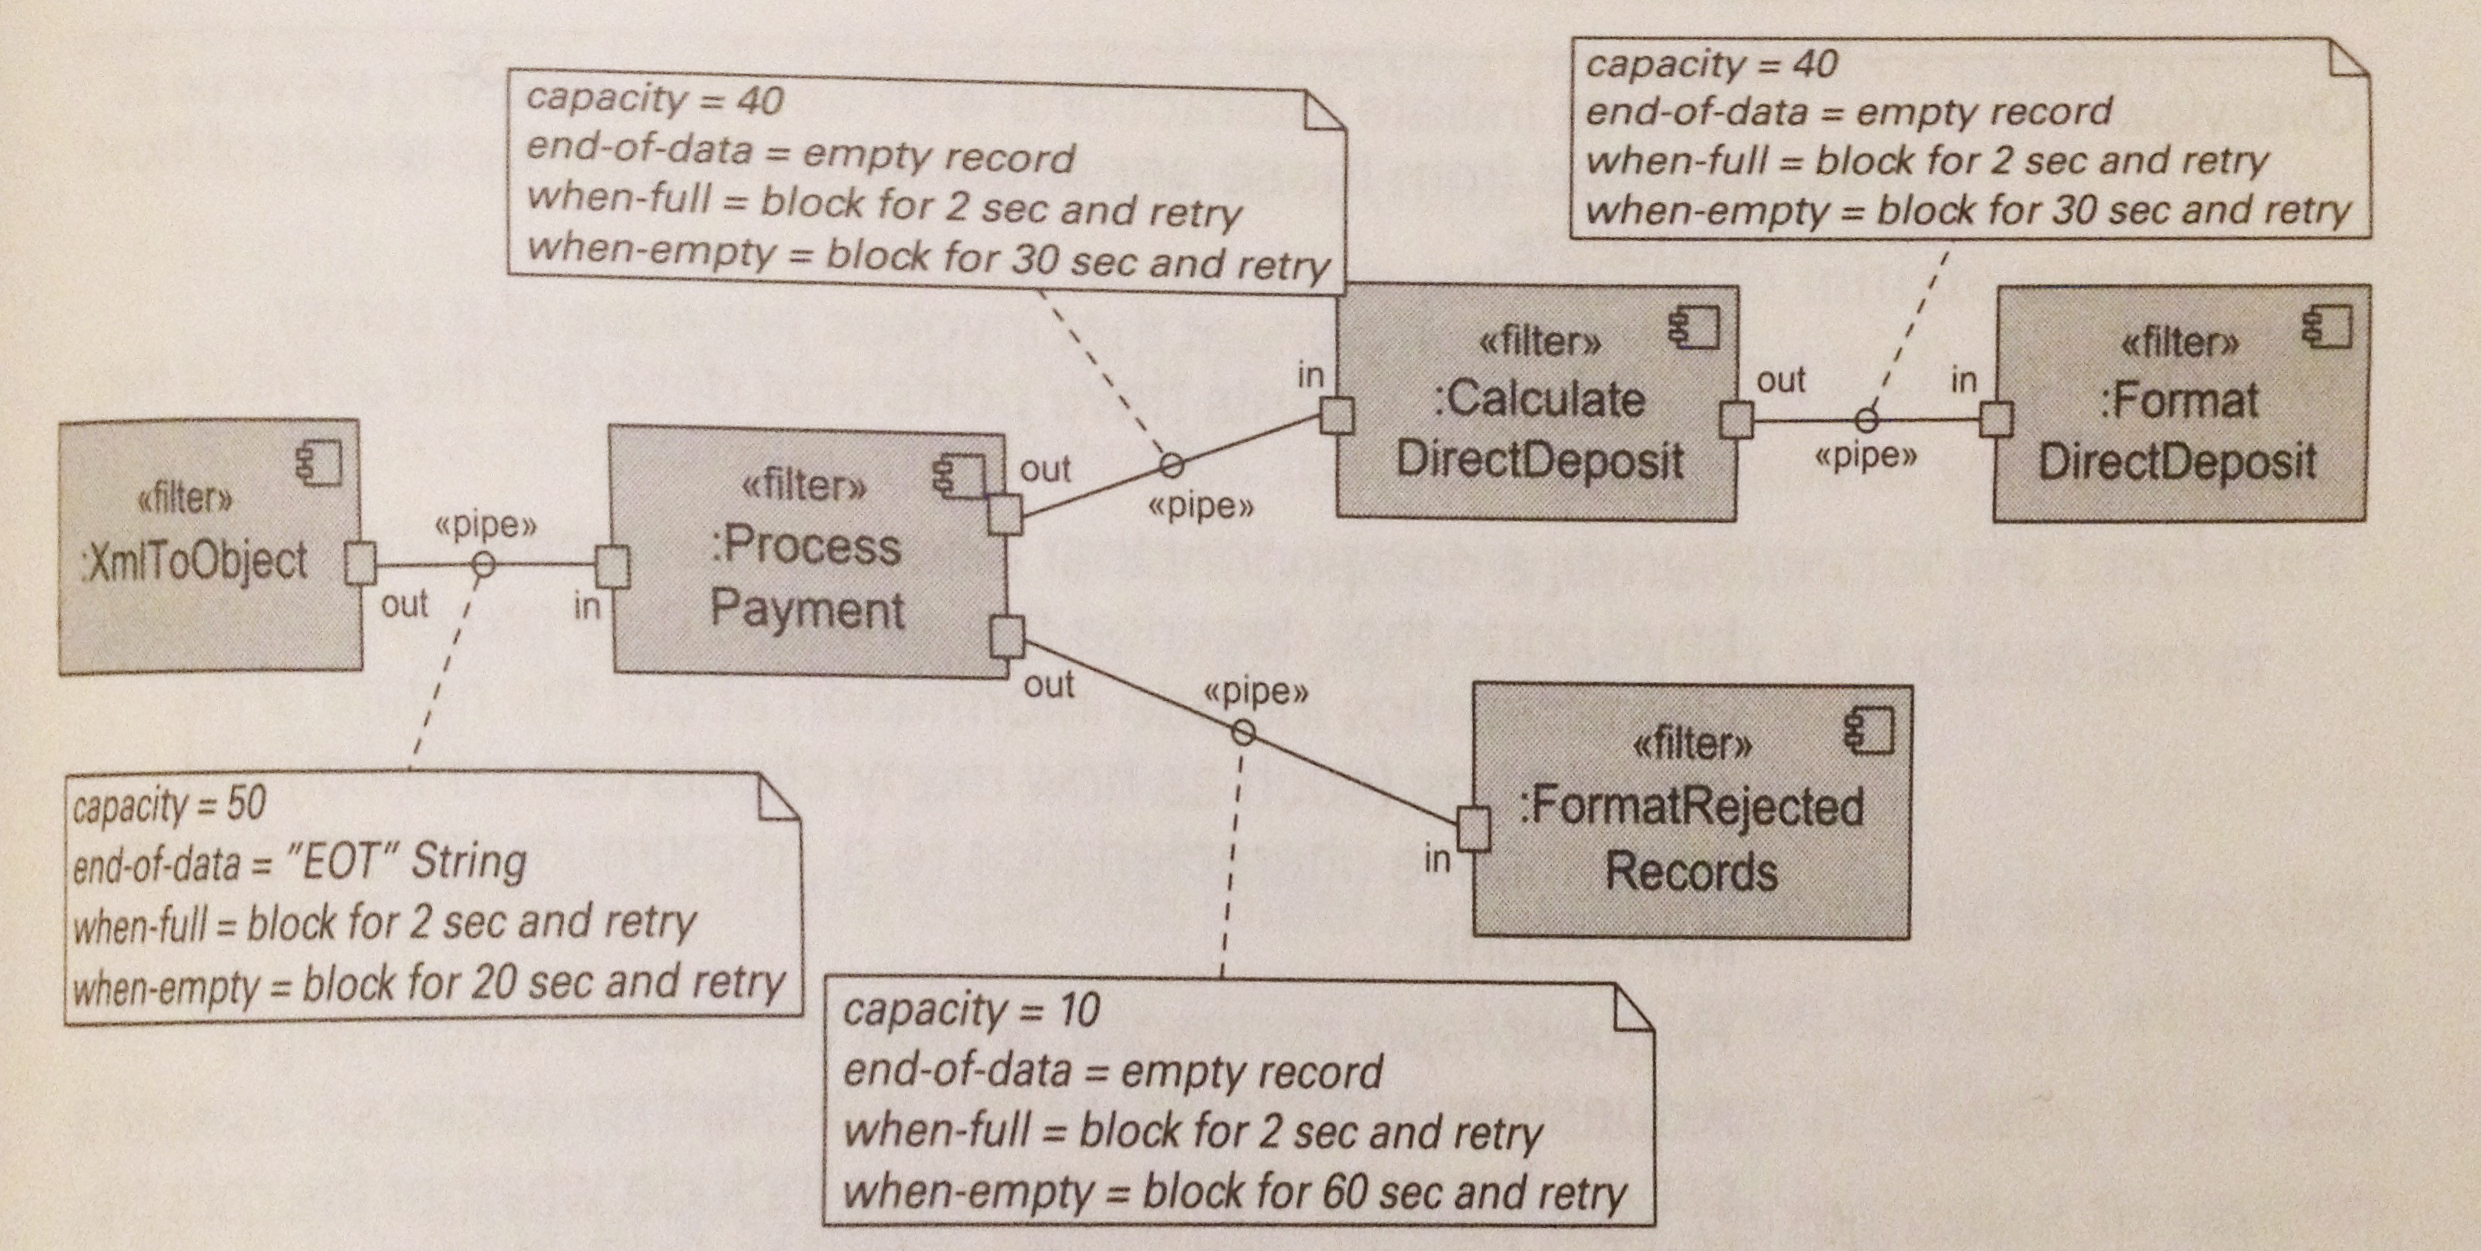
\includegraphics[width=\textwidth/2,center]{pipes-and-filters.png}
	\caption{The pipe-and-filter-pattern. \cite[p. 217]{bass2012software}}
	\label{fig:pipeandfilter-pattern}
\end{figure}

The \textit{layered} pattern is a way to provide a separations of concern
(segmentation between modules) in a complex system. This allows modules to be
developed and modified separately, without changing other modules. This relies
on principle that each layer provides a stable interface. Normally in a layer
architecture each layer can communicate only with the next (lower) layer. There
are however many violations to the pattern made for trade-off reasons, usually
performance. According to Bass et al.. it is one of the most commonly used 
patterns in software engineering. \cite[pp. 205-210]{bass2012software}

The \textit{multi-tier} pattern is often used to distribute a system into
distinct subsets. It is often used when different software components are
running on different physical nodes. Each tier represents a logical grouping of
components. One computing node can run multiple tiers, but still communicate
through a defined interface between the nodes. Tiering adds a level of
abstraction that introduces overhead and increases system complexity, but the
trade-offs include increased modifiability and reduces coupling.
 \cite[pp. 235-238]{bass2012software}

\section{Related Research}
\label{background:rel_reasearch}
The majority of research related to motorsport is related to design and
construction; very little research has been performed with the goal of giving
the driver a better environment. Most of the research done on driver
environments and IVIS is focused on safety. Lim et al. \cite{lim1999heads}
tested a prototype HUD-solution in a snow plow with focus on low visibility
conditions. Cheng et al. \cite{cheng2007intelligentVehicles} tested drivers
ability to follow the speed limit when aided by a HUD-display. A collision 
warning and traffic monitoring system was tested on military vehicles by
Nishizawa et al. \cite{nishizawa1997heads}, which in addition to a HUD also
used sounds to alert the driver. Cottle et al. \cite{wirelessDashboard}
designed a wireless ``dashboard'' built into a steering wheel in a Formula
Student car, but very little focus was put on the end user experience. There
has also been done some studies on the effect of distractions on driver response
time, both cognitive \cite{visualDistractionsStudy} and physical 
distractions \cite{hancock1999effects} have been studied.

Goeble et al. \cite{goebl2007realtimecapable}
developed an architecture that supported interchange of information with
different temporal resolution between computing nodes in cognitive automobiles.
The system is very large and complex and is made to support exchange of
information between multiple consumers and producers with either hard or soft 
real-time requirements.

Stewart et al. \cite{stewart1993integration} developed a framework that
utilized a global state table with a single lock to facilitate information 
exchange in reconfigurable sensor-based control systems. Although the paper is
from 1993 it is still relevant to our application, however the inter-component communication described is significantly
different from the serial buses utilized in modern cars.

In their 1995 paper Magee et al. \cite{magee1995specifying} presents the 
Darwin notation for specifying the architectural level of distributed 
systems. Darwin is an architecture description language (ADL), another ADL is
Wright \cite{Allen97Thesis}. ADLs are used to formally describe software architectures.
Despite their common goals, Allen \cite[p. 24]{Allen97Thesis} argues that Darwin
``does not provide an adequate basis for analysis of the behavior of an
architecture.''.



\endgroup %Resets chapter page-shifting before next chapter :)
 % and state of the art
%% !TEX root=../thesis.tex
\chapter{Method}
\label{chapter:method}

In working with this project the group has undertaken a considerable study of
literature around both software architecture, software metrics and assessment, electronics, display technology,
and studies about driver environments and performance. The literature has
served as a platform to support our project goals of creating an enabling
software architecture. The group has also conducted an interview with a driver
from last years Revolve-team. In collaboration with Revolve we have elicited
requirements and use-case scenarios which in turn has resulted in our proposed
architecture design (including design artifacts) and assessment guidelines.

The biggest weakness of the architecture described herein is the lack of
verification. First, during the project period we didn't have access to any hardware
similar to the one the system will be running on. Second, there are still some
uncertainties with regards to the amount of data that is to be handled by the
system due to the fact that sensor update rates and CAN-bus package format is
still an unknown factor. We have however developed a proof-of-concept desktop
application to simulate a configuration environment for the proposed system.
We will be discussing this application further in \vref{chapter:results}. 

\section{Literature Study}
To acquire a broad picture of the problem area and domain the group has studied
a varied set of literature ranging from research articles to books on various topics. Some of the most useful literature we have read includes the following:
\begin{itemize}
	\item ``An Introduction to Object-Oriented Analysis and Design and Iterative Development'' by Craig Larman \cite{Larman:UML}
	\item ``Software Architecture in Practice'' by Bass, L. and Clements, P. and Kazman, R.
	 \cite{bass2012software}
	\item ``Designing embedded hardware [Kindle Edition]'' by John Catsoulis
	\item ``A software architecture evaluation model'' by Dueñas, Juan C and de Oliveira, William L and Juan, A.
	\cite{duenas1998software}
\end{itemize} 
For an exhaustive list of all literature used we refer to the
bibliography\vpageref{bibliography}.

\section{Architecture Design Method}
In the process of designing this architecture we have opted to use design
artifacts and methods described by Craig Larman \cite{Larman:UML}. We started
out at the beginning with performing an interview with one of last years 
drivers (\vref{interview:bakkom}) to get a picture of how the cockpit 
experience is for the driver during
an event. We also got some interesting ideas to build on. Building on this
information we arranged an informal requirements workshop together with a few 
members of this years Revolve-team; eliciting both quality requirements and
functional requirements (and lots of ambitious ideas). One important benefit of
bringing experienced members in on the workshop was that we could easily
discover external requirements originating in the FS competition rules \cite{fsae:2014rules}.
Both Larman and Bass et al. suggests that a systems
architecture should be based mostly on non-functional and quality requirements,
especially those that strongly influence the architecture.
\cite[p.20]{bass2012software}\cite[pp. 541-554]{Larman:UML}

After the workshop we started working on refining and defining the results,
writing up use-cases in a terse format. Larman suggests \cite[pp. 95-95]{Larman:UML}
that during early phases of development most use cases (except the ones that 
might be architecturally significant or with high risk) should be kept terse 
and rather be expanded upon and refined when development is underway. Since no
architectural development was performed during this project we decided to spend
more time trying to clarify them and use the results to help with identifying
the architectural requirements.

In the further process we listed the discovered requirements in an
architectural factors table \cite[pp. 56-59, 545-547]{Larman:UML}. The goal of
this activity was to define measures that can be used to measure the
architecture's ability to meet the goals and requirements, and to give an
easily accessible ranking of importance for these requirements.

The last artifact to be developed was the system architecture document \cite[p. 550]{Larman:UML} where we
recorded and detailed the suggested solutions, and their reasoning, to resolve the architectural
factors.

In working with the architecture design we have tried to work in an iterative
fashion, but due to the compact nature of the project some processes bear the
look and feel of a ``waterfall'' process. We do not intend that the
architectural design suggestion presented in this project to be the final one, 
but rather its intended to be a good
starting point for development and refinement. We also suggest metrics that can
be used to measure if the architecture meets the goals set, and believe it is important
that the control process starts early in the development to see if the
architecture meets the requirements or needs further work 
\cite[pp. 556-557]{Larman:UML}.

In describing our architecture we have opted to use UML, or modeling close to
UML where we felt that it increased readability, or where we were pressed for time and
UML compliance wasn't deemed the most important, planning to revise this when
further development is being undertaken. We chose to not use any ADLs to describe the
system, in part because that would be worthy a project of its own, and in part because we 
are not interested in traces of the system 
\cite[p. 42-43]{Roscoe:2005:TPC:550448},
but in the systems ability to meet its critical requirements. 




%% !TEX root=../thesis.tex

\chapter{Results}
\label{chapter:results}

\section{List learned, to be removed} % (fold)
\label{sec:list_learned_to_be_removed}

\begin{itemize}
	\item Important characteristics
	\begin{itemize}
		\item Stakeholders 
		\begin{itemize}
			\item Defined relevant stakeholders in a hierarchy for more easy 
			aggregation (stakeholder awareness).
			\item Defined requirements of the stakeholders (what information 
			do they need)
			\item Clearly defined responsibility area per level in hierarchy (
			example in data sets)
		\end{itemize}
		\item Data sets
		\begin{itemize}
			\item Information stored accordingly to stakeholders
			\begin{itemize}
				\item In this case as example, stations defined per 
				responsibility area
				\item Other info is connected to stakeholders through
				stations, for clarification of connected to:
				\item Other info is connected to stakeholders through stations, for clarification of connected to
				see following 3 points:
				\item For crossings between trains, compares on equal 
				station at the same time
				\item Density is between given stations
				\item This means stations are stored per area, and other 
				info is fetched according to this.
			\end{itemize}
			\item Generalize data storage
			\begin{itemize}
				\item Easier to remove or add more data to a data set
				\item When having generalized data storage and generalized 
				aggregation, it means it is much easier to add other type of data sets
			\end{itemize}
		\end{itemize}
		\item Aggregation
		\begin{itemize}
			\item Generalize methods for reuse throughout the hierarchy levels and
			through different types of information
			\begin{itemize}
				\item This could mean generating equal return data structure regardless of
				stakeholder hierarchy level and type of data
				\item Results in a much more general information display
				\item Aggregate over data on the step between data storage and presentation
			\end{itemize}
			\item Aggregate through data from different sources
			\item When the data is relative simple (read for instance count per station), a simple aggregation is averaging the data through different stakeholder hierarchy
			level.
			\item Data presentation view based on current selected stakeholder 
			which in turns determines what should be aggregated and returned to be
			presented
		\end{itemize}
		\item Data retrieval optimization
		\begin{itemize}
			\item Minimize data traffic
			\item Efficient queries to minimize execution time
			\item Generality in storage and queries for scalability both  
			in size and data types needed
			\item External vs local storage?
			\item All in one or independent data storage per information 
			type?
		\end{itemize}
		\item Navigation through time and space
		\begin{itemize}
			\item Have a selectable time intersection for limiting data view
			\item "Zoom" the data in space based on the responsibility area/needs of the stakeholders, in this case, fit the visible section of the map to the relevant stations
		\end{itemize}
	\end{itemize}
\end{itemize}

% section list_learned_to_be_removed (end)

% !TEX root=../../thesis.tex

\section{Workshop 2014-04-04} % (fold)
\label{sec:workshop_2014_04_04}
The first workshops agenda was to help define the stakeholders of the system,
their areas of responsibility, and their needs. The workshop was also meant to 
bring clarity to how the system will relate to these users and their needs.
Attending this workshop was Andreas Amdal Seim (SINTEF), Andreas Dypvik 
Landmark (SINTEF), Rimmert van der Kooij (SINTEF), Nils Olsson (NTNU), Per 
Magnus Hegglund (Jernbaneverket), Magnus Bae (NTNU), and Magnus Krane (NTNU).\\

Perspectives that can be used when viewing the system were discussed
first.
\begin{itemize}
	\item Infrastructur: Segment director, etc.
	\item Traffic division / passenger / train companies.
	\item Delay causes: delay demographic.
\end{itemize}

Interests of users when using the system were then discussed based on the
perspectives.
\begin{itemize}
	\item Uptime, punctuality.
	\item Deviation.
	\begin{itemize}
		\item What?
		\item Where?
		\item When?
	\end{itemize}
	\item Delay time.
	\item Variation.
	\item Changes.
\end{itemize}

Causes that might affect the punctuality was also listed: weather, number of
passengers, capacity utilization, animal accidents, cargo volume.
The causes was concluded not to be included in this project, as the causes is
difficult to prove and get data on.\\

The internal project in Jernbaneverket (section
\Ref{sub:subsection_jernbaneverket}) uses a deviation registry for data to
analyze each stretch on a detail level. To calculate the uptime, presented in
\Ref{sec:railway_operations}, also uses the deviation registry for the needed
data. A problem by using the deviation registry for calculating variation or 
changes, the registry have a five minute filter in which the trains are being 
calculated to be on time.

Two problems were agreed upon that needed to be addressed, the back end and 
the  front end of the system. What kind of data is available and what is 
possible to do with this data? A data set can show both positive and negative 
results, based on what the set are compared too. For instance, easter is not 
on the same week each year and the passenger volume increase during the 
holidays. Data sets ended up being addressed in the second workshop (\Ref{sec:workshop_2014_04_24}). 

As the different stakeholders might have need for different presentation of the
data, different levels of stakeholders and what should be shown in each level 
was discussed. A suggestion was made to have the same perspective through the
levels, but to have selectable views based on roles. \\

At the end of the workshop, three conclusions was made. The first conclusion 
was to have a dashboard next to each marker with relevant data to the current 
stakeholder. The second conclusion was to a interactive list of the
stakeholders which adapted the visual presentation to the selected stakeholder,
presented in \Ref{sec:back_stakeholders}.
The last conclusion was to have a second workshop where the content of the
dashboard should be decided. This resulted in \Ref{sec:workshop_2014_04_24}.

% section workshop_2014_04_04 (end)

\section{Workshop 2014-04-24} % (fold)
\label{sec:workshop_2014_04_24}
The second workshops agenda was to determine what statistical data was 
to be implemented in the dashboard, concluded upon in \Ref{sec:workshop_2014_04_04}.
Attending this workshop was Andreas Amdal Seim (SINTEF), Andreas Dypvik 
Landmark (SINTEF), Rimmert van der Kooij (SINTEF), and Magnus Krane (NTNU).\\

The workshop started with a brainstorming for different data to present in
the map. The different data was ranked on implementation practicality from 1 - 
3 where 1 is unpractical and 3 is very practical; and ranked on the 
desirability of the data from 1 - 3 where 1 is undesirable and 3 is very 
desirable. The brainstorming after ranking is presented in \Ref{table:dashboard_functionality_wants_vs_needs}.
\\

\begin{table}[!h]\small
	\begin{tabularx}{\textwidth}{|X|l|l|l|}
		\hline
		Functionality & Practicability & Desirable & Priority\\
		\hline
		Outstanding errors & 1 & 1 & 1\\
		\hline
		Suspensions & 3 & 1 & 3\\
		\hline
		Variation & 1 & 3 & 3\\
		\hline
		Season effects & 3 & 1 & 3\\
		\hline
		Follow delays & 1 & 3 & 3\\
		\hline
		Speed limits & 3 & 1 & 3\\
		\hline
		Cause & 3 & 2 & 6\\
		\hline
	 	Worst stretch/station/train number & 3 & 2 & 6\\
		\hline
		Delays & 3 & 3 & 9\\
		\hline
		Traffic density & 3 & 3 & 9\\
		\hline
		Speed restrictions & 3 & 3 & 9\\
		\hline
		Crossings & 3 & 3 & 9\\
		\hline
	\end{tabularx}
\caption{Dashboard functionality brainstorming ideas}
\label{table:dashboard_functionality_wants_vs_needs}
\end{table}

Based on the ranking, the decision was made to only implement the data was
ranked as a 3 both on practicability and desirability, presented in the list
below.

\begin{itemize}
  \item Speed restrictions
  \item Crossings
  \item Traffic density
\end{itemize}

The second part of the agenda, was to determine how the selected data was to be
presented. The decision was made to split the presentation in two parts. The
first was to display aggregated data in the dashboards next to the marker based
on the current stakeholder. The second was to display top 5 lists for delays
and speed restrictions.

\subsection{Crossings} % (fold)
\label{sub:crossings}
One of the problems discussed with crossing was should the system take into 
account the difference between actual crossings and planed crossings or not? 
The difference is hard to calculate as one does not know whether one of the 
trains involved in the planned crossing, was canceled or just delayed. The 
decision was made to present the number of crossings occurred at each station, 
and aggregate the number as one navigates in the stakeholder hierarchy.
%TODO planned crossings, ask Landmark.
% subsection crossings (end)

\subsection{Traffic density} % (fold)
\label{sub:traffic_density}
Several options to present traffic density were discussed, the problem was how
to correctly show the number of trains based on the data available. 
Should the system present each train based on the train numbers and 
calculate for the entire line both ways? Should the system display train 
numbers divided by the segment directors? 

In the workshop it was decided to show the number of trains that passes each 
block segment, based on the data available. When navigating in the hierarchy,
the system shall aggregate the number of trains.

% subsection traffic_density (end)

\subsection{Speed restrictions} % (fold)
\label{sub:speed_restrictions}
Speed restrictions was decided to be presented a marker per restriction, and be
shown between the selected time interval. The data for the speed restrictions
was to be presented in a plot which appeared in the marker for each
restriction.

%In the dashboard it was decided to show the top 5 upper and lower bounds. It was also decided to include a little marker on the map to indicate the location of the speed restriction. 

% subsection speed_restrictions (end)

% section workshop_2014_04_245 (end)

% section workshops (end)


%\section{Prototype} % (fold)
%\label{sec:prototype}
%In this section we will describe how the developed prototype implemented the
%problem of the research question.
%
%\begin{itemize}
%	\item What are important characteristics for a stakeholder aware method to 
%	aggregate over a rich set of data?
%\end{itemize}
%
%When a important part of the system is to be aware of stakeholders and their
%requirements and needs, we found it important to have a easy way of selecting 
%different stakeholders. By having this selection,  We presented this in \Ref{sub:front_end_aggregation}.

% section prototype (end)

%% !TEX root=../thesis.tex
\chapter{Discussion}
\label{chapter:discussion}

\section{Stakeholders and aggregation} % (fold)
\label{sec:discussion_stakeholders_and_aggregation}
It is important to define the needs and requirements of the stakeholders early 
in the process, in order to design a system that gives the right scope. By the 
aid of workshops we defined the requirements, as it is part of the research 
method (see \Ref{sec:workshops}). We can define the stakeholders in a 
hierarchy, based on their organizational structure, and responsibility areas, 
this helps us to define the requirements to order the structure of the 
information.

There is a good synergy between the requirements and the system, when the 
system is designed with the requirements in mind. The synergy between the 
requirements and the system both have advantages and disadvantages. On one 
side the system has a great possibility to satisfy the requirements and needs 
of the stakeholders, since the system is tightly connected to the 
requirements. On the other side, the system can be inflexible to large 
changes, if the requirements change late in the project. In the workshops, we 
defined that the stakeholders must have the ability to view different kinds of 
information; the system must take these needs into consideration. A system 
aware of the stakeholders needs might end up being more complex, and has to 
process a larger amount of data in order to give the system the required 
functionality. Processing larger amounts of data leads to a more complex back-
end system. The system can be more dynamic, although complex, by reusing parts 
of the data processing for different information types, when designed with the 
needs as well as the requirements in mind. In order to meet the requirements 
of the stakeholders needs we have to aggregate the data. There are several 
ways to aggregate the groups of data according to the given criteria. 
Discussion can be around the method we used for the aggregation of the data, 
which enables the best view for the stakeholders. For the best view we take 
into account for example the following alternatives: average, minimum, 
maximum, median, and count. To decide the aggregation method, we have to 
consider how each information type is structured, but also how this structure 
fits in with the stakeholder their hierarchy. During the workshops, we decided 
that the best way to aggregate the data is to take the average, the decision 
was based on how the data is connected to the stakeholders and their
hierarchy.

When returning the processed data to the user, the system can use the 
requirements to aggregate the presentation of the data. Since the stakeholder 
their hierarchy contains the responsibility area of each stakeholder, the 
system can fit the visual view to the responsibility area of the current 
stakeholder. The system uses processed data for aggregating the hierarchy to 
find the stakeholder. Fitting the view to the stakeholder provides detail for 
a single stakeholder, this is useful for presenting a single stakeholder and 
their responsibility area. Since the system is aware of the stakeholders,
aggregating for a stakeholder and fitting the view to a stakeholder, can lead
to a conflict of interest between stakeholders and occurs due to overlapping 
responsibility areas. The conflict is extremely difficult to consider when
presenting the data and is therefor not taken into consideration. We decided 
to fit the visual presentation of data to the current stakeholder, and have 
the opportunity to jump, back and forth, within the hierarchy of the
stakeholders. By fitting the view to the stakeholder, the view enabled the 
user to receive more relevant information on the current stakeholder.

As the area director wants to study data from the entire area for a large 
period of time, and the segment director wants to study almost every detail 
that occurs on the segment, manual navigating in time was decided to use as a 
way to increase and decrease the level of detail in the data presented.


Keywords:

\begin{itemize}
	\item Important to define requirements early, in order to make an appropriate system, that is useful for the stakeholders
	\item How to define the stakeholders and requirements for use with a system?
	\begin{itemize}
		\item important to define who are the stakeholders
		\item important to define what the stakeholders needs are
		\item important to define to which need are connected to which stakeholder, in order to show the correct information in the system connected to each of the stakeholders needs.
	\end{itemize}
	\item How can we design a system that used the requirements needed by the stakeholders to process the data and visualize the data in such a way that the stakeholders needs are met?
	In order to meet the requirements of the stakeholders needs we need to aggregate the data. The following .....
	\item aggregation of data:
	\begin{itemize}
		\item two goals: geographic \& time
		\item aggregation based on detail level of visualization
		\begin{itemize}
			\item based on stakeholders need
			\begin{itemize}
				\item detail level in map
				\item which area is shown in the map
				\item aggregation based on time
			\end{itemize}
		\end{itemize}
	\end{itemize}
	\item Data aggregation methods
	\begin{itemize}
		\item What are good ways to aggregate the data?
		\item How to determine what fits the requirements?
	\end{itemize}
	\item How to present the data to the users based on the requirements? (detail
	level per stakeholder in the hierarchy)
	\item Time navigation for zooming through the data.
\end{itemize}


% section stakeholders_and_aggregation (end)

\section{Data storage and data queries} % (fold)
\label{sec:discussion_data_storage_and_data_queries}
By having several types of information which have different structure and
originating from different sources, the question of how the data storage should
be structured gets raised. One option for the structure is to merge all the
data sets into one large database. When the data is stored in one large
database
 When having one large, merged 
database, one experiences little maintainability, which is the degree where a
product or system can be modified by the intended maintainers\cite[p. 195]{Bass:2012:SAP:2392670}. 
One large database also means that we avoid duplication of data.
Another way to structure the data storage is to store the data sets in
independent storages with a loose coupling between the structures. Since most 
changes to a system happens after initial release, as described by Bass, 
Clements, and Kazman \cite[pp. 117-124]{Bass:2012:SAP:2392670},
means that when the data sets are designed with built-in flexibility, 
exercising the built-inn flexibility is usually cheaper than to hand-
code a specific change in hindsight. By having these loosely linked data sets,
one have achieved a modifiable data storage. This thesis demonstrated this
principal by having the stations stored in a hierarchy data set based one the 
stakeholder hierarchy, and the other data sets connected to the stations.\\



Keywords:
\begin{itemize}
	\item Data set structure in prototype
	\begin{itemize}
		\item How should the data sets be structured when the sets are based 
		on the stakeholders need for different type of information?
		\begin{itemize}
			\item Connection to the requirements of the stakeholders.
			\begin{itemize}
				\item Stakeholder responsibility area from the hierarchy
			\end{itemize}
			\item Advantages and disadvantages with one or several sets in storage.
			\begin{itemize}
				\item Scalability and modifiability ref quality attributes \cite{Bass:2012:SAP:2392670}
				\item Duplication of data with several sets of data.
			\end{itemize}
		\end{itemize}
	\end{itemize}
	\item Data queries
	\begin{itemize}
		\item Limit queries for data processing efficiency 
		and more responsive systems
		\begin{itemize}
			\item By the aid of time navigation and requirements, limit the 
			queries for more efficient calls to the data storage.
			\item The system will be more efficient in the processing of the 
			data, when limiting the quires.
		\end{itemize}
		\item Front end vs back end data processing for system efficiency and
		limiting data traffic
		\item Should the data be processed in the front-end or the back-end 
		of the system?
		\begin{itemize}
			\item The data should be aggregated in the back-end of the system, 
			since it is more efficient.
			\begin{itemize}
				\item Quicker calls to the database from the back-end.
				\item Less data traffic during transfer of.
				\item Usually quick hardware on server side, while it have a 
				great span in the front-end.
			\end{itemize}
		\end{itemize}
	\end{itemize}
\end{itemize}
% section data_storage_and_queries (end)

\section{Review of own work} % (fold)
\label{sec:review_of_own_work}
%Keywords:
%\begin{itemize}
%	\item Appropriate method?
%	\item 
%\end{itemize}
% section review_of_own_work (end)

%% !TEX root=../thesis.tex
\chapter{Conclusion and Future work}
\label{chapter:conclusion}

\section{Conclusion} % (fold)
\label{sec:conclusion}
Fill out based on List of learned, started in \ref{sec:characteristics}:
% section conclusion (end)

\section{Future work} % (fold)
\label{sec:future_work}

Suggestions of things to do:
\begin{itemize}
	\item dynamic top 5 list
	\item difference actual and planned crossings
	\item Affecting contexts
	\item Freight volum, passengers, capacity utilization, etc
\end{itemize}
% section future_work (end)

% !TEX root=../../thesis.tex

\section{Characteristics} % (fold)
\label{sec:characteristics}
This will mainly be melted inn conclusion and results. Was meant for typing out
list in \Ref{sec:list_learned_to_be_removed}.

\textbf{Research question}
\begin{itemize}
	\item What are important characteristics for a stakeholder aware method to 
	aggregate over a rich set of data?
\end{itemize}

When one needs a method that are aware of stakeholders for aggregating, it is
important to have a clearly defined hierarchy of the stakeholders and their 
responsibility area. When implementing the stakeholder hierarchy in the
developed prototype, it was implemented as a selectable list in the upper right
corner, see \Ref{fig:stakeholder_selection_list}. This means that when 
one wants to move in the hierarchy, one simply clicks their way through the list to the wanted area.


Since by navigating through the stakeholder hierarchy by selecting different
levels in the selectable list means that the aggregation logic in the 
background determines what is displayed, it provides a good example of
displaying information based on what fits the needs of the current stakeholder.
When the display receives the return data, it fits the view of the map to
data. When sending queries the map also sends along time data, from user 
inputs. This time data, is taking into consideration with the stakeholder when 
determining what kind of data should be returned and displayed.\\

Since the data is stored in sets, it is possible to do a intersect on the data
based on the requirements of the stakeholder and the selectable time data.
By combining these two, one is able to navigate through the  data both in time 
and space and it is possible to limit the information displayed at any given
time based on the needs of the stakeholder.\\

%XXX visualiser med Venn-diagram\\

Since the methods that shall aggregate over the data sets have to to consider
both the stakeholder and the data type, the methods should be dynamic so that
they can be reused throughout every stakeholder and every type of data. To 
achieve this dynamic, one should have loosely linked data with stakeholders
such as that the data sets are easily editable in terms of adding or removing
data, or adding new type of data sets.

Since most of the statistical data used in this thesis, are sorted on one 
identifier and that identifier is connected to the stakeholders, there are 
quite easy to expand the data sets. This means that the aggregation is actually
a three step process.

\begin{description}
	\item [1. Identify stakeholders needs] By searching the set of data that 
	have the connection to the stakeholders based on a given stakeholder, one 
	is able to generate a list of all the identifiers relevant to this 
	stakeholder.
	\item [2. Retrieve relevant data] By using the the list of relevant
	identifiers generated based on the stakeholder, one is able to find all 
	wanted data.
	\item [3. Aggregate through the found data] When one have acquired the 
	wanted data, one aggregates through the data according to the 
	specification of that set of data.
\end{description}


By having a loosely linked storage of the different data sets, an important
thing to take into consideration is optimization of Step 2 listed above. Since
one is able to navigate through time as described, the system is able to limit
the amount of data it has to process at each execution. By adding clauses which
will limit the result, the query time will drop and the performance time of the
aggregation will improve, both in terms of waiting for returning data from
queries on the data sets and with processing said data.\\

By having the user selecting the wanted stakeholder and what type of
information the system shall present, it enables the system dynamically
determine which data set it shall look in and aggregate through. This is
demonstrated in \Ref{fig:stakeholder_selection_list} which is the
selection of stakeholders and in \Ref{fig:implementation_type_selection} is the selection of data
sets.

Since the aggregation methods by this point have received wanted stakeholders,
the wanted type of information to be display according to the stakeholders
needs, and time interval for limiting the data set, the aggregation should now
be able to generate the correct data according to the stakeholders
requirements. The methods should then, according to step 2 retrieve the data
and loop through it according to the requirements. As was demonstrated in this 
prototype, most data was a simple count of occurrences. This meant then when
aggregation through the responsible areas of each stakeholder it was a mostly
done by averaging all occurrences beneath that area and generating a dummy
marker for each sub-area with the aggregated data of that area.


% section characteristics (end)



\label{bibliography}
\bibliography{bibliography}
%\nocite{*} %All
%\nocite{key1,key2,keyN}

%Use ieeetr to get correct numbering of references according to the IEEE
% standard. Numbering follows order of introduction.
\bibliographystyle{ieeetr}


% Header for appendices
%\chapter{Appendices}
%    \begin{center}
%    \topskip0pt
%    \vspace*{\fill}
%     This page intentionally left blank     %   Nice and centered :D
%    \vspace*{\fill}
%    \end{center}

%\appendix
%\setcounter{page}{0}
%\pagenumbering{roman}
%% !TEX root=../thesis.tex

\chapter{Theory}

In this appendix we look at --- meh!

\subsection{Types of systems}
In general there are basically two types of driver information systems, Heads Down Display and Heads Up Display. 
The first is represented by the classic we all know; the dashboard. The second we find in more advanced 
applications such as in fighter planes where the pilot wears a helmet with a display in the visor. In the latter 
example the operator has a display that is fixed in position, but because the helmet moves with head movement, so does
the display. In the first example the display is fixed and operator head and eye movement is required to use the display during normal
operation.

Revolve have always chosen to utilize dashboard-based information systems. Mainly consisting of LED-displays and 
LED-indicators. To get an insight into the efficiency of these systems we conducted an interview with a driver 
from the 2013-competitions. During this interview we learned that during a race it is very hard to consume
information from the dashboard. The course twists and turns, and requires the driver to focus on track and on handling the car; braking and 
acceleration. This makes it difficult for the driver to shift focus down to the dashboard and usually requires longer straight sections of
track to be able to gather any meaningful information.



% \subsection{Scope}
% The scope of this project is to research the state-of-the-art of 
% HUD-technology. What type of devices and technology that can 
% be leveraged to create a prototype HUD for application in a racing car. 
% Focusing both on the racing parts of the competition, and on helping
% to win points in the business side of the competition. (link to background chapters)

% \subsection{Application}Incorporating a HUD-system in a race car is something that could provide a competetive advantage. For Revolve NTNU 
% this is doubly so, since the Formula Student competetion covers so many disiplines the advantages given may also contribute to better 
% results in business-class competitions. (link to background chapter here)
 %maybe we should find something useful to put here
% before we include it ^^

%\addtocontents{toc}{\protect\setcounter{tocdepth}{0}}

%\chapter{Interviews}
\clearpage

\section*{Driver interview}
\label{interview:bakkom}
Date: 2013-09-25\\
Subject: Ole Edvard Bakkom\\
Interviewers: Magnus Krane and Magnus Bae\\
\\
The purpose of of this interview was two-fold: (1) To gain knowledge about what types
of information that a Formula Student class racecar-driver consumes during typical events 
under an FS-competion. (2) To discuss what type of information that would be feasible for the driver
to consume in different circumstances; racing, training, renting a high performance vehicle for a limited time.


\begin{dialogue}
    \speak{Magnus} During a race how much information do you manage to consume from the instrument panel? 
    \speak{Ole} Not much, maybe a blinking LED or two, but it's difficult to read the speedometer for instance. 
    	The pace is quite high, and very few straights. This makes it difficult to be able to look down
    	and focus on complex information. 
    \speak{Magnus} Do you think you'd be able to consume more information in competitive context if the information was 
    	presented in a way that you didn't have to shift your focus away from where you're looking, for instance a heads-up-display?
    \speak{Ole} Yes, I think that would be a considerable improvement over last year's solution, as long as it's not obtrusive.
    	Although the usage in the competition might be a bit limited, I think it could be amazing for testing.
    \speak{Magnus} How do you think it would contribute in testing?
    \speak{Ole} Well, there's lots of things, but the first that comes to mind is, since we're building an electric car this year,
    	charging level - to get a notification when the battery needs to be charged or battery percentage.\\
    	Second the ability to have two-way communication with the rest of the crew. Last year we had to stop whenever they wanted to
    	give a message.\\
    	Lap-times would definitively make a difference during testing. Previously we've had to wait until we switched drivers to get a list of our lap times.\\
    	Cone-hits, in the competition we get added times for every cone we hit(flip?), getting real-time or close to it feedback if we hit a cone would be very practical.
    \speak{Magnus} What about in the competition? Which of these would be important? Two-way communication maybe?
    \speak{Ole} In the competition we're not allowed to have two-way communication with the vehicle or driver. The vehicle is allowed to send, but not receive.
    	With reservations that they might have changed the rules for 2014.
    \speak{Magnus} So no two-way communication. Can you think of anything that could be valuable for the competion?
    \speak{Ole} Well, we're adding brake pressure adjustment, and showing data or settings for it could be very practical. Using data from wheel sensors
    	maybe you could show an alert if a wheel locks up as well, hinting the driver to adjust brake balance
    \speak{Magnus} Interesting, I'm automatically thinking Gran Turismo 5-style info. Basically graphics showing the four tires, and changing color to red
    	when one locks up.
    \speak{Ole} That could work. There's also been talk about monitoring tire temperature using infrared sensors.
    \speak{Magnus} There's also the business case; rental for the weekend-racing. What type of information do you think could be interesting in that
    	context, something that would sell well with the judges? We've been thinking about creating an optimal route for the track using GPS, and then showing deviance.
    \speak{Ole} That sounds like a good idea. How about showing ghost data? Best or last lap would be really cool. I think that would really make testing better too. 
    	If you could have a laptimer showing as well that would be a good motivator. 
    \speak{Magnus} Maybe having real-time difference between previous (or best) lap could work as well? And how about sectoring it, comparing on a corner-per-corner basis
    	 
    \speak{Ole} Definitely. If I could compare myself lap by lap I would definitely push myself harder. Trying out different racing lines and corner speeds would give 
    	instant feedback. That's something that I think would really be cool, both for training and the business case.\\
    	Using GPS-data, could you show optimal speed through a corner? If you know the layout of the track that could probably calculated? Alternatively comparing speeds through
    	corners with your own best speed. 
    \speak{Magnus} Interesting. Calculating theoretical optimum speed might be far from reality? How about giving achievments if your laptime is 13 seconds and 37 hundreds?
    	
    \speak{Ole} Hehe, achievments could be cool. Even if the calculated max speed is off you'd get an indication. If you go through a corner at 50 and max speed 
    	could be 70 it should mean that you can push harder.
    \speak{Magnus} Good point. How about drifting, showing you how far you drifted around a corner?
    \speak{Ole} The cars don't really drift well, but maybe showing if you're close to optimum slip could be quite nice. Maybe a G-diagram, 
    	showing how much G's you're getting through corners. 
    \speak{Magnus} Noted. Could be cool, using data from accelerometers maybe. So if you were to prioritize, what would you put as the number one
    	priority? 
    \speak{Ole} That would definitively be for testing, lap times and indication of difference is what I think would add the most value during testing and training.
    \speak{Magnus} Ok. What do you think would be the biggest benefits of such a system?
    \speak{Ole} I think one benefit would be that it would make testing more effective. Second, it could make it much easier to push your own performance. 
    \speak{Magnus} Thank you for the interview, I feel we've gotten a lot of insight and good ideas here. If you think of anything else please let us know. 
    \speak{Ole} I will see if I can come up with something. 
    
  \end{dialogue} 


  The interview transcript was approved by Ole Edvard Bakkom on 2013-10-10.

%% !TEX root=../thesis.tex

\chapter{The Formula Student Competitions}
\label{appendix:formula}
\clearpage
The Formula Student competitions is a series of international competitions 
between engineering students where teams compete with small formula-style cars 
they have designed and built from scratch:

\begin{quote}
Your team is tasked to produce a prototype for a single-seat race car for auto-cross or sprint racing, and 
present it to a hypothetical manufacturing firm. The car must be low in cost, easy to maintain, and reliable, with high 
performance in terms of its acceleration, braking, and  handling qualities. During the competition your team must demonstrate 
the logic behind your proposal and must be able to demonstrate that it can  support a viable business model for both parties.
 \cite{FS:challenge}
%(http://www.formulastudent.com/formula-student/about-us/thechallenge)
\end{quote}

\noindent Any FS competition is built up with 3 static and 5 dynamic events. The static events is where the teams must defend their design 
and solutions on the car; why the car has cost as much or little as it did, and try to sell it to investors through a 
business plan. The dynamic events is meant to test the abilities of the car in both cornering and acceleration, 
durability, and fuel-efficiency.

\section{Static Events}
Engineering Design Event: 
An eight page Design Report is being reviewed by the judges followed by an inspection of the constructions and discussion 
with the students. This is where the teams defend every part of the car. Why designs, parts, etc. were chosen. 
A maximum of 150 points can be awarded. \cite{FSG:disciplines}

Cost and Manufacturing Event:
Based on the Cost Report, which details the cost of the prototype, the teams discuss every aspect of the car with the judges 
why the cost estimate ended up as it did. The cost report is based on a list of all components, where every item has a cost 
based on what the part is made of, how it is made, and how it is put together. These are not the real costs of the part, but
synthetic and standardized values close to the cost that would be incurred during manufacturing. A maximum of 100 points can be awarded. \cite{FSG:disciplines}

Business Presentation Event:
 The team gives a 10 minute presentation where the judges pretend to be representatives of a fictional manufacturer  and the 
 point is to show that the car is suited for the target group (nonproffesional weekend autocross racing). During this 
 presentation the focus is on value and sell-ability. A maximum of 75 points can be awarded. \cite{FSG:disciplines}
  %cite{http://www.formulastudent.de/fsg/about/disciplines/}

\section{Dynamic Events}
Acceleration: This is where the car's acceleration gets tested. The event is based on a straight line race on 75 meters of track. A maximum 
of 75 points can be awarded. \cite{FSG:disciplines}

Skid-pad: This event tests how much lateral acceleration the cars can produce. The course is built in the shape of a figure of eight. 
The car goes round each circle twice and the last of the rounds on each circle is timed, the total time is the average of those 
two times. A maximum of 100 points can be awarded. \cite{FSG:disciplines}

Auto-cross: The auto-cross event tests the cars driving dynamics and handling qualities. 
The cars race on a one kilometer course composed of straights and curves.
A maximum of 100 points can be awarded. \cite{FSG:disciplines}

Endurance: This event tests the durability of the car over a 22 kilometer long course. Every aspect of the cars physical capabilities 
gets put to the test during this event, such as acceleration, handling and reliability. A maximum of 325 points can be awarded. \cite{FSG:disciplines}

Fuel efficiency: The fuel efficiency of the car is calculated based on average fuel consumption per completed lap. This event is calculated 
based on the endurance event, and the teams must complete the driver exchange before the fuel efficiency is allowed to be 
calculated. A maximum of 100 points can be awarded. \cite{FSG:disciplines}\\

%% !TEX root=../thesis.tex
\chapter{System requirements}
\label{requirements}

In this chapter we present the requirements for a driver information system for Revolve NTNU.

\section{Non-functional requirements} %they're also non-fictional.

The system
\begin{itemize}
	\item Shall deliver information to the driver with less than 200 ms delay 90\% of the time.
	\item Shall not negatively affect the drivers performance.
	\item Shall not obstruct the drivers entry or exit from the vehicle.
	\item Shall connect to the car's CAN-bus system.
	\item Shall not interfere with the normal operating of the car's CAN-bus system.
	\item Shall convert received sensor values to real-world values.
	\item Shall help Revolve NTNU obtain their goals in the FS competitions.
	\item Shall support easy removal or addition of new sensors and equipment
\end{itemize}

\section{Functional requirements} %These are fictional
The system
\begin{itemize}
	\item Shall not deliver old information in the case of loss of one or more inputs.
	\item Shall deliver information about the current speed.
	\item Shall deliver information about the current battery charge level.
	\item Shall warn if the current battery charge level is running below critical threshold\footnotemark[1].
	\item Shall warn and alert if the battery temperature has passed a critical threshold\footnotemark[1].
	\item Shall deliver information about lap times after lap is completed if lap-timing system is operational.
\end{itemize}

%footnotes
\footnotetext[1]{This value is unknown at the time of writing and will be defined at a later point}



%\chapter{Vision Document}
%\label{appendix:vision}
%\includepdf[link,pages={-}]{output/vision.pdf}
%
%
%\chapter{System Requirements Document}
%\label{appendix:requirements}
%\includepdf[link,pages={-}]{output/requirements.pdf}
%
%
%\chapter{Supplementary Specification Document}
%\label{appendix:supspec}
%\includepdf[link,pages={-}]{output/supspec.pdf}
%
%\chapter{System Architecture Document}
%\label{appendix:sad}
%\includepdf[link,pages={-}]{output/architecture.pdf}

%\include{acronyms}
%\section{Attachments}
	\label{sec:attachments}

\subsection{U file for hydraulic piston case.}
\subsection{p file for hydraulic piston case.}
\subsection{pointMotionU file for hydraulic piston case.}
\subsection{blockMeshDict file for for hydraulic piston case.}

\subsection{U file for dynamic simulation of the concentric cylinder case.}
\subsection{p file for dynamic simulation of the concentric cylinder case.}
\subsection{pointDisplacement file for dynamic simulation of the concentric cylinder case.}
\subsection{blockMeshDict file for dynamic simulation of the concentric cylinder case.}
\subsection{controlDict file for dynamic simulation of the concentric cylinder case.}
\subsection{forces file for dynamic simulation of the concentric cylinder case.}

\subsection{angularOscillatingDisplacementPointPatchVectorField.C file.}
\subsection{oscillatingDisplacementPointPatchVectorField.C file.}
\subsection{libMyFunctionDisplacementPointPatchVectorField.C file.}

\subsection{Matlab script for generating .dat file for use in pointMotionU file.}
\subsection{pointDisplacement file for use with modified library.}
\subsection{Matlab script for plotting of analytical solution for pressure gradient.}
\subsection{Matlab script for autogeneration of simulated velocity profiles.}
\subsection{Matlab script for autogeneration of simulated force plots.}
%\includepdf[pages={-}]{} Legge til pdf


\end{document}
